%!TEX root = Main.tex
\vspace{-0.1in}
\section{Case for a global name service}
\label{sec:case}

Given the huge body of prior work specifically on mobility as well as more broadly on Internet architecture, it is natural to  begin by asking:  Is a global name resolution service critical to handling mobility if we had the luxury of refactoring Internet naming and routing from a clean slate? %In this section, we first present subjective arguments to justify an affirmative position on this question, and then describe DNS's shortcomings as a resolution service under high mobility for today's Internet.

%justifying an affirmative position on both questions, and then present objective results showing DNS's shortcomings as a resolution service under high mobility.

%(1) is a global name resolution service the best way to handle high mobility in today's Internet?

\subsection{Internet mobility background}

\label{sec:bg}



%An enormous body of prior research has focused on re-architecting Internet naming and routing in part to enhance support for mobility. Table \ref{tab:arch} classifies a number of proposed architectural alternatives based on how they handle mobility. Although the list is but a representative sample and many of the listed designs are driven by goals beyond just mobility, the classification helps us appreciate the pros and cons of the small number of fundamentally different known approaches to handle mobility. 

Despite a staggering diversity of proposals re-architecting Internet naming and routing, we find that they explicitly or implicitly embed one of three broad approaches to handling mobility--{\em indirection-based routing, global name-to-address resolution}, or {\em name-based routing}--based on how they go from the name of an endpoint to the endpoint itself.

%Several internet naming and routing architectures have addressed the problem of enhancing support for mobility in the Internet. 


%Many of these works include eloquent discourses on the architectural ills of the Internet, pointing to location-identity conflation as the prime accused and the lack of seamless support for mobility as Exhibit A. In this section, we reflect on this body of work offering a less fashionable perspective, namely that despite a large number of alternative naming and routing architectures, we only know of a small number of fundamentally different ways of handling mobility; the original Internet was not that far off the mark; and what is needed both in the current Internet as well as many of the alternative proposals is a practical resolution infrastructure that can quickly resolve mobile identifiers to network locations at Internet scales.

\eat {

\begin{table*}[t]
\centering
\small{
\begin{tabular}{|p{0.98in}|p{1.4in}|p{2.2in}|p{1.7in}|}
\hline
 %Approaches  $\rightarrow$ 
 
 %Design traits $\downarrow$ 
 & {\bf Indirection-based routing} & {\bf Global name-to-address resolution} & {\bf Name-based routing} \\
  \hline
  Initial overhead & None & Name-to-address resolution (DNS, Nimrod\cite{Nimrod}, LISP\cite{LISP}, HIP\cite{HIP}, LNA\cite{LNA}, CoDoNS\cite{codons-paper}, XIA\cite{XIA}, MobilityFirst\cite{MobilityFirst-UMASS}) & None\\
  \hline
  Data packet routing &  
 {Address-based routing through fixed ``home address'' (Mobile IP\cite{MIP}, GSM\cite{GSM}, i3\cite{i3})}
  & Address-based routing, with support for late- or re-binding of names to addresses (e.g., Serval \cite{serval}, MobilityFirst\cite{MobilityFirst-UMASS}, XIA\cite{XIA})
 %, HAIR\cite{HAIR}, AIP\cite{AIP}, XIA\cite{XIA}, MobilityFirst\cite{MobilityFirst}
	 & 
	 {Name-based routing directly over flat (ROFL \cite{ROFL}) or structured names (TRIAD\cite{TRIAD}, CCN\cite{CCN})}\\
\hline
%Routing data plane & Address-based  & Address-based
%& Name-based  with optional underlay addressing (DONA\cite{DONA}, Serval\cite{serval}) \\ 
%\hline
Mid-connection-mobility handling &  Seamless in one RTT & 
Bilateral (\cite{Migrate},\cite{ECCP}) or via name service (under concurrent mobility) in a few RTTs
& 
Outage times $\approx$ routing convergence delays
\\  
\hline
Routing table size vs. data path stretch &  O(\#prefixes) with triangle routing stretch & O(\#prefixes) or O(\#domains) (\cite{XIA}, \cite{MobilityFirst-UMASS}) for shortest-path routing & 
$\Omega$(\#identifiers) for small stretch over shortest-path routing \cite{compact-routing}
\\
%No aggregation: $\Omega$(N) for constant stretch over shortest-path \cite{compact-routing}.

%With aggregation: O(\# ``displaced'' identifiers)\\
 \hline
\end{tabular}
}
\vspace{-0.15in}
\caption{Classification of many alternative naming and routing architectures (not necessarily designed with mobility in mind) based on how they (might) handle mobility.}
\vspace{-0.1in}
\label{tab:arch}
\end{table*}

}

\newcommand{\indirection}{indirection-based routing}
\newcommand{\Indirection}{Indirection-based routing}
\newcommand{\Logcen}{Global name-to-address resolution}
\newcommand{\logcen}{global name-to-address resolution}
\newcommand{\namerouting}{name-based routing}
\newcommand{\Namerouting}{Name-based routing}

{\textbf \Indirection} schemes are simple as an endpoint remains oblivious to the mobility of other endpoints. No name-to-address\footnote{We use the terms {\em name} and {\em identifier} interchangeably; likewise for the terms {\em address} and {\em location}.} lookup is needed at connection initiation time as a human-readable name maps to a {\em home address} (an IP address in Mobile IP \cite{MIP} or a flat identifier's consistent-hash location in i3 \cite{i3}) that rarely changes by design. Mid-connection mobility, even when both endpoints move concurrently, is seamless to endpoints. However, the data plane pays the price for this simplicity---every data packet must be routed via an indirection agent at the home address, potentially causing significant routing stretch, e.g., two participants at a conference may in each direction need to detour packets halfway across the world despite being in the same  room. %In the case of i3, routing stretch is incurred both at the overlay DHT layer (to reach a rendezvous point) in addition to stretch in the data plane because of mobility, so the authors suggest several alternatives to optimize this stretch  (e.g., choosing the closest of several rendezvous points;  caching IP addresses to handle the conference room scenario, etc.). 
%Mobile IP's sender-oblivious design works well for mobility but is forced to either offer an inflexible design for multihoming or sacrifice sender-obliviousness.  
Furthermore, indirection-based schemes require widespread deployment of indirection agents across different domains, posing a barrier to immediate adoption.

{\textbf \Logcen} schemes rely on a distributed service %that is distinct from the underlying network
to resolve names to addresses as the first step in connection establishment. The current Internet's DNS as well as a number of designs addressing the Internet's so-called identity-location conflation problem also need such a resolution infrastructure, e.g., to translate a self-certifying host identifier in HIP \cite{HIP}, AIP\cite{AIP}, XIA\cite{XIA}, or MobilityFirst\cite{MobilityFirst-UMASS}) or an identifier in LISP \cite{LISP} or HAIR \cite{HAIR} to either an IP address \cite{HIP}, a self-certifying network identifier \cite{AIP,XIA,MobilityFirst-UMASS}, or a hierarchical locator \cite{HAIR} that encodes routing information. \Logcen\ schemes also subsume DHT-based Internet architectures such as LNA \cite{LNA,DOA} %or others \cite{DOA,UIP} 
as well as resolution systems like CoDoNS \cite{codons-paper} that present a DHT-based drop-in replacement for DNS.

%Proposals such as Layered Naming Architecture (LNA) \cite{LNA} or closely related architectures (e.g., DOA \cite{DOA}, UIP\cite{UIP}) recommend overlay DHT routing to translate flat identifiers (or EIDs) to the IP address of the destination. Generally (and as explicitly advocated by LNA), only the first packet in the connection needs to rely on DHT routing to locate the destination as it is more efficient to send subsequent data directly to the destination's IP address, falling back to the DHT in case of an error, say, because of mid-session mobility. Thus, the DHT is essentially a logically centralized, physically distributed, overlay name resolution service replacing DNS. Indeed, systems like CoDoNS \cite{codons-paper} present a DHT-based design as a drop-in replacement for DNS. 

{\Logcen} schemes need explicit  support at endpoints to handle mid-connection mobility. There is a general consensus \cite{Migrate,ECCP,TCP-R} that end-to-end connection migration, i.e., bilaterally without relying on an external service,  suffices to migrate connections efficiently when endpoints move one at a time, but an external resolution service is needed to support concurrent mobility. Although the latter is seen as a rare case in most connection migration work, it can be common in disconnection-tolerant, mobile application scenarios, e.g., when a user closes her laptop at home and opens it at a coffee shop to continue watching a movie, by which time the cloud-hosted virtual server may have been migrated for load balancing.

{\textbf \Namerouting} schemes in the ideal have a tantalizing intellectual lure---to seamlessly handle mobility by routing directly over names  with no resolution step---but are marred by several fundamental and practical challenges. First, \namerouting\ approaches can support seamless mobility only if routing update propagation delays are on the order of milliseconds, a daunting challenge given that interdomain routing can take several minutes to converge today. Second, theoretical results on compact routing \cite{compact-routing} suggest discouraging fundamental trade-offs between the size of forwarding tables at routers and path stretch even without any mobility or multihoming, e.g.,  routing over N flat identifiers entails a prohibitive $\Omega(N)$ forwarding table size per router in order to ensure a small constant stretch factor ($\approx$3) compared to shortest-path routing. Simulation-based studies of flat-label routing strategies (e.g., ROFL \cite{ROFL}) reaffirm pessimistic conclusions about its scalability. 

Although it may appear that the scalability limitations of name-based routing can be alleviated by adding a hierarchical structure to names \cite{TRIAD, DONA, CCN} (e.g., NDN-style \cite{CCN} names such as  \verb+/umass/phone42/call3/frame7+), frequent mobility still poses a challenge as routers would have to maintain special forwarding entries for ``displaced names'', i.e., names that move from their hierarchically organized namespace (say, from \verb+/umass+ to \verb+/comcast+ in this example) for longest-prefix matching to work correctly. That is, high mobility effectively makes routing directly over structured names as hard as routing over flat names unless indirection or a name resolution infrastructure is used, a conjecture that has recently been empirically reinforced by Gao et al. \cite{Gao14LocInd}.

\eat {
 as an endpoint will be unreachable immediately after it has moved to parts of the network that haven't yet received routing updates. For example, in order to handle frequent mobility in NDN, either most routers need to maintain separate forwarding entries for ``displaced'' names, e.g., when \verb+john_smith_phone+ above moves from the \verb+/umass+ to the \verb+/comcast+ network, so that longest-prefix matching ensures reachability, or the routing layer has to rely on indirection via a ``home'' network (e.g., as advocated by \cite{MobileIP-like-approach-for-CCN})\footnote{A disclaimer: The designers of NDN themselves are strictly agnostic to strategies to handle high mobility but have suggested that they are open to the option of augmenting NDN with a global name resolution infrastructure \cite{personal-comunications-at-FIA-meetings} to assist routing. }
As most mobile users spend a significant fraction of each day displaced from any reasonable definition of a ``home'' network (e.g., residential ISP, workplace, etc.), displaced names will entail a prohibitive overhead either in forwarding table sizes or path stretch, i.e., high mobility effectively makes routing directly over structured names as hard as routing over flat names.
}

%An early example of this approach is TRIAD \cite{TRIAD} that proposed routing directly over name spaces as opposed to address prefixes, an idea that is also central to the more recent CCN \cite{CCN} (or NDN \cite{NDN}) approach that advocates eliminating addresses altogether. ROFL \cite{ROFL} aims even higher seeking to route over completely flat names, but the authors report pessimistic conclusions about its scalability. Approaches like DONA \cite{DONA} or Serval \cite{serval} seek to provide an abstraction of flat-name routing on top of an IP-address-based underlay (but are classified as network-layer because they tightly integrate routing and name-to-address resolution). On paper, network-layer schemes promise seamless mobility, multihoming, and anycasting to the nearest location, but face the following challenges in practice.


%advocate a more radical alternative, namely to handle mobility completely at the network layer obviating a name resolution infrastructure. For example, TRIAD \cite{TRIAD} was one of the earliest to propose routing directly on name spaces instead of IP address prefixes, an idea that is also central to the more recent CCN \cite{CCN} (or NDN \cite{NDN}) architecture that adopts a more purist stance eliminating interface addresses altogether. Designs such as DONA \cite{DONA} and Serval \cite{serval} route on flat identifiers using a ``resolution handler'' or ``service routing'' plane on top of an underlying IP network. ROFL \cite{ROFL} adopts a more purist approach routing directly on flat identifiers in the underlying network, but the authors report mixed or pessimistic conclusions about its scalability. A key strength of network-layer approaches is that an endpoint can remain oblivious to the mobility of other endpoints, however this strength comes with several caveats.

{\bf{Summary.}} Our position is that a \logcen\ service is critical for handling high mobility in any network architecture as it offers the best combination of trade-offs: (1) a constant update overhead per mobility event to the name service, (2) a modest connection establishment overhead and rapid mid-connection mobility, (3) no data path inflation beyond underlying policy routing, and (4) small forwarding table sizes in conjunction with aggregatable addresses (IP prefixes like today or self-certifying network addresses \cite{MobilityFirst-UMASS,XIA}). Perhaps the most compelling argument for  \logcen\ is our decades of familiarity with DNS and the Internet; handling mobility would be a drop-in replacement to DNS provided we address the challenge of building a distributed system that scales to billions of devices making many updates a day and yet returns up-to-date responses within milliseconds. %Addressing this challenge is the focus of the rest of this paper.

\subsection{Limitations of DNS}
\label{sec:whyNotDNS}

\blue{
What specific design traits of DNS make it poorly suited for mobile applications? The first two traits below limit its scalability with respect to the rate of endpoint mobility, and the third limits its scalability with respect to the size of the namespace if applications were to have the luxury of using arbitrary (but fixed) names.
}

\blue{ 
(1) {\em TTL-based caching:} TTL-based caching is the single-most important mechanism for DNS's scalability; caching not only helps DNS sustain essentially arbitrarily high {\em lookup load} but also dramatically reduces client-perceived {\em lookup  latency} for cache hits. However, caching is ineffective when TTLs are near-zero, as would have to be the case under high mobility, causing both increased load on name servers and higher client-perceived latencies. Caching is also less effective if lookups are distributed relatively uniformly, as could be the case with mobile device names, unlike lookups for today's domain names that are highly skewed \cite{Jung, DHTdns}.
}

\blue {
(2) {\em Static placement:} Authoritative DNS servers are essentially rendezvous points that allow a mobile endpoint to inform potential correspondents of its current location(s). In order to reduce the time-to-connect, authoritative servers must be located close to potential correspondents. However, authoritative server locations today are static, either close to a mobile endpoint's ``home'' location or a pre-packaged set of geo-distributed locations provided by a managed DNS provider. Engineering a scalable geo-distributed system that can dynamically move object replicas in a demand-aware manner is nontrivial and real-world examples of such systems have only recently begun to emerge \cite{spanner}.
}

%\blue{
(3) {\em Hierarchical names:} The hierarchical structure of DNS names is key to leveraging {\em federation} to scale to an arbitrary {number of names} by delegating different portions of the name space (or {zones}) to different organizations. For example, root name servers today only have to maintain state for a small number of top-level domain names.  In contrast, arbitrary or flat names, e.g., ``\verb+JohnSmith3142's watch+'' can not be supported in DNS while retaining the scaling benefits of federation as the root name servers would have to maintain nonzero state, e.g., at least the authoritative name server(s) and the DNSSEC key of a name, for essentially all names. Our position is that the design of a general-purpose global name service must not restrict the structure of names as names carry application-specific semantics; in $\S$\ref{sec:context}, we show examples of novel context-aware communication primitives that are feasible with unrestricted names.
%}

\blue{
{{Our approach}} to address the first two issues above relies on {\em active} and {\em demand-aware} replication: (1) Active replication significantly reduces (but does not eliminate) the reliance on passive caching; (2) Demand-aware replication ensures that active replicas of a name record are accessible close to clients querying the name, so as to reduce the overall {time-to-connect}. A glib but pedagogically helpful way to highlight the difference from DNS is that, in the extreme case, our approach can create an active replica of a name record near every DNS local name server that stores a passively cached copy today. Our approach addresses the third issue above by cleanly separating resolution of names from adjudication and certification. We explain our approach in detail next.
}


























%%%%%%%%%%%%%%%older version from conext'13 %%%%%%%%%%%%%%%%%%

\eat{
\subsection{Internet mobility background}

An enormous body of prior research has focused on re-architecting Internet naming and routing in part to enhance support for mobility. Table \ref{tab:arch} classifies a number of proposed architectural alternatives based on how they handle mobility. Although the list is but a representative sample and many of the listed designs are driven by goals beyond just mobility, the classification helps us appreciate the pros and cons of the small number of fundamentally different known approaches to handle mobility. We find that existing approaches can be broadly classified as {\em indirection-based, logically-centralized}, or {\em network-layer} based on how they go from the name of an endpoint to its location, as we elaborate below.

%Several internet naming and routing architectures have addressed the problem of enhancing support for mobility in the Internet. 


%Many of these works include eloquent discourses on the architectural ills of the Internet, pointing to location-identity conflation as the prime accused and the lack of seamless support for mobility as Exhibit A. In this section, we reflect on this body of work offering a less fashionable perspective, namely that despite a large number of alternative naming and routing architectures, we only know of a small number of fundamentally different ways of handling mobility; the original Internet was not that far off the mark; and what is needed both in the current Internet as well as many of the alternative proposals is a practical resolution infrastructure that can quickly resolve mobile identifiers to network locations at Internet scales.

\begin{table*}[t]
\centering
\small{
\begin{tabular}{|p{1in}|p{1.2in}|p{2.2in}|p{2in}|}
\hline
 Approaches  $\rightarrow$ 
 
 Design traits $\downarrow$ & {\bf Indirection-based} & {\bf Logically-centralized} & {\bf Network-layer} \\
  \hline
  Initial name-to-address lookup &  
 {None as home address fixed by design (Mobile IP\cite{MIP}, GSM\cite{GSM}, i3\cite{i3})}
  & Distributed overlay (DNS, Nimrod\cite{Nimrod}, LISP\cite{LISP}, HIP\cite{HIP}) including  {DHT-based} schemes (LNA\cite{LNA}, CoDoNS\cite{codons-paper})
 %, HAIR\cite{HAIR}, AIP\cite{AIP}, XIA\cite{XIA}, MobilityFirst\cite{MobilityFirst}
	 & 
	 {None as network supports name-based routing abstraction (TRIAD\cite{TRIAD}, ROFL\cite{ROFL}, CCN\cite{CCN})}\\
\hline
Routing data plane & Address-based  & Address-based

& Name-based  with optional underlay addressing (DONA\cite{DONA}, Serval\cite{serval}) \\ 
\hline
Mid-session-mobility  (delay) &  Seamless (1RTT) & 
  
Bilateral end-to-end (\cite{Migrate},\cite{ECCP}) + name service for concurrent mobility (few RTTs)

& 
Seamless (outage times $\approx$ routing convergence delays)
\\  
\hline
|Routing table| v. data path stretch &  O(\#prefixes) with triangle routing overhead & O(\#prefixes) or O(\#domains) (XIA\cite{XIA}, MobilityFirst\cite{MobilityFirst-UMASS}) for shortest-path & 

$\Omega$(\#identifiers) for small stretch over shortest-path \cite{compact-routing}
\\
%No aggregation: $\Omega$(N) for constant stretch over shortest-path \cite{compact-routing}.

%With aggregation: O(\# ``displaced'' identifiers)\\
 \hline
\end{tabular}
}
\vspace{-0.15in}
\caption{Tripartite classification (indirection-based, logically-centralized, network-layer) of many alternative naming and routing approaches based on how they handle mobility.}
\vspace{-0.1in}
\label{tab:arch}
\end{table*}


{\em Indirection-based} schemes are simple as an endpoint remains oblivious to the mobility of other endpoints. No name-to-address\footnote{We use the terms {\em name} and {\em identifier} interchangeably; likewise for the terms {\em address} and {\em location}.} lookup is needed at connection initiation time as a human-readable name maps to a {\em home address} (an IP address in Mobile IP \cite{MIP} or a flat identifier's consistent-hash location in i3 \cite{i3}) that rarely changes by design. Mid-session mobility, even when both endpoints move concurrently, is seamless to endpoints. However, the data plane pays the price for this simplicity---every data packet must be routed via an indirection agent at the home address, potentially causing significant routing stretch, e.g., two participants at a conference may in each direction need to detour packets halfway across the world despite being in the same  room. %In the case of i3, routing stretch is incurred both at the overlay DHT layer (to reach a rendezvous point) in addition to stretch in the data plane because of mobility, so the authors suggest several alternatives to optimize this stretch  (e.g., choosing the closest of several rendezvous points;  caching IP addresses to handle the conference room scenario, etc.). 
%Mobile IP's sender-oblivious design works well for mobility but is forced to either offer an inflexible design for multihoming or sacrifice sender-obliviousness.  
Furthermore, indirection-based schemes require widespread deployment of indirection agents across different domains, posing a barrier to immediate adoption.

{\em Logically-centralized} schemes rely on a distributed service that is distinct from the underlying network to resolve names to addresses as the first step in connection establishment. The current Internet's DNS as well as a number of designs addressing the Internet's so-called location-identity conflation problem also need such a resolution infrastructure, e.g., to translate a self-certifying host identifier in HIP \cite{HIP} (or AIP\cite{AIP}, XIA\cite{XIA}, MobilityFirst\cite{MobilityFirst-UMASS}) or an identifier in LISP \cite{LISP} or HAIR \cite{HAIR} to either an IP address \cite{HIP}, a self-certifying network identifier \cite{AIP,XIA,MobilityFirst-UMASS}, or a hierarchical locator \cite{HAIR} that encodes routing information. Logically centralized schemes also subsume DHT-based Internet architectures such as LNA \cite{LNA} or others \cite{DOA,UIP} as well as resolution systems like CoDoNS \cite{codons-paper} that advocate a DHT-based design as a drop-in replacement for DNS.

%Proposals such as Layered Naming Architecture (LNA) \cite{LNA} or closely related architectures (e.g., DOA \cite{DOA}, UIP\cite{UIP}) recommend overlay DHT routing to translate flat identifiers (or EIDs) to the IP address of the destination. Generally (and as explicitly advocated by LNA), only the first packet in the connection needs to rely on DHT routing to locate the destination as it is more efficient to send subsequent data directly to the destination's IP address, falling back to the DHT in case of an error, say, because of mid-session mobility. Thus, the DHT is essentially a logically centralized, physically distributed, overlay name resolution service replacing DNS. Indeed, systems like CoDoNS \cite{codons-paper} present a DHT-based design as a drop-in replacement for DNS. 

Logically centralized schemes need explicit  support at endpoints to handle mid-session mobility. There seems to be a general consensus \cite{Migrate,ECCP,TCP-R} that end-to-end or bilateral connection migration, i.e., without relying on an external service, suffices as an efficient approach to migrating connections when endpoints move one at a time; however, a centralized lookup service is needed to support concurrent mobility. The latter is seen as a rare case in most connection migration work, however it can be a common event for disconnection-tolerant, mobile application scenarios (e.g., a user closes her laptop at home and opens it at a coffee shop to continue watching a streaming movie, by which time the cloud-hosted server may have been migrated for load balancing).

{\em Network-layer} schemes promise an academic ideal---to seamlessly handle mobility by routing directly over names obviating a name resolution infrastructure---but are marred by several fundamental and practical challenges. An early example of this approach is TRIAD \cite{TRIAD} that proposed routing directly over name spaces as opposed to address prefixes, an idea that is also central to the more recent CCN \cite{CCN} (or NDN \cite{NDN}) approach that advocates eliminating addresses altogether. ROFL \cite{ROFL} aims even higher seeking to route over completely flat names, but the authors report pessimistic conclusions about its scalability. Approaches like DONA \cite{DONA} or Serval \cite{serval} seek to provide an abstraction of flat-name routing on top of an IP-address-based underlay (but are classified as network-layer because they tightly integrate routing and name-to-address resolution). On paper, network-layer schemes promise seamless mobility, multihoming, and anycasting to the nearest location, but face the following challenges in practice.


%advocate a more radical alternative, namely to handle mobility completely at the network layer obviating a name resolution infrastructure. For example, TRIAD \cite{TRIAD} was one of the earliest to propose routing directly on name spaces instead of IP address prefixes, an idea that is also central to the more recent CCN \cite{CCN} (or NDN \cite{NDN}) architecture that adopts a more purist stance eliminating interface addresses altogether. Designs such as DONA \cite{DONA} and Serval \cite{serval} route on flat identifiers using a ``resolution handler'' or ``service routing'' plane on top of an underlying IP network. ROFL \cite{ROFL} adopts a more purist approach routing directly on flat identifiers in the underlying network, but the authors report mixed or pessimistic conclusions about its scalability. A key strength of network-layer approaches is that an endpoint can remain oblivious to the mobility of other endpoints, however this strength comes with several caveats.

First, network-layer approaches can support seamless mobility only if routing update propagation delays across the Internet are on the order of milliseconds, a daunting challenge given that interdomain routing can take several minutes to converge today. Second, and more importantly, theoretical results on compact routing \cite{compact-routing} suggest discouraging fundamental trade-offs between the size of forwarding tables at routers and path stretch even without any mobility and multihoming, e.g.,  routing over N flat identifiers entails a prohibitive $\Omega(N)$ forwarding table size in order to ensure a small constant stretch factor ($\approx$3) compared to shortest-path routing.  This overhead can be alleviated by adding a hierarchical structure to names (e.g., provider\_id: device\_id in DONA, or CCN names such as  \verb+/umass/john_smith_phone/voip_call3/frame7+). But frequent mobility poses a challenge as a mobile endpoint will be unreachable immediately after it has moved to parts of the network that haven't yet received routing updates. Furthermore, most routers would need to maintain separate forwarding entries for ``displaced'' names, e.g., when \verb+john_smith_phone+ above moves from \verb+/umass+ to \verb+/comcast+, so that longest-prefix matching ensures reachability.
As most mobile users spend a significant fraction of each day displaced from any reasonable definition of a ``home'' network (e.g., residential ISP, workplace, etc.), the forwarding table overhead induced by such displaced names is likely to be prohibitive, i.e., frequent mobility makes routing over structured names as hard as routing over flat names.

In {summary}, we posit that all mobility approaches must either rely on a logically centralized resolution service in order to scale, or adopt an indirection-based approach and inherit their drawbacks. A logically centralized approach offers the best combination of traits: (i) a small update overhead per mobility event to the name service, (ii) efficient mid-session mobility, (iii) no data path inflation beyond underlying policy routing, and (iv) small forwarding table sizes in conjunction with aggregatable network addresses (IP prefixes like today or self-certifying network addresses \cite{MobilityFirst-UMASS,XIA}).
 Perhaps the most compelling argument for the logically-centralized approach is our decades of familiarity with DNS and the current Internet; handling mobility would be a drop-in replacement to DNS provided we can address the challenge of building a distributed system that can scale to billions of devices making tens of updates a day and yet return responses within a few milliseconds. Addressing this challenge forms the focus of the rest of the paper.

}



%%%%%%%%%%%%%% Older version below from sigcomm'13 submission.

\eat {
An enormous body of prior research has focused on re-architecting Internet naming and routing in order to enhance support for mobility, multihoming, content retrieval, or security. Many of these works include eloquent discourses on the architectural ills of the Internet, pointing to location-identity conflation as the prime accused and the lack of seamless support for mobility as Exhibit A. In this section, we reflect on this body of work offering a less fashionable perspective, namely that despite a large number of alternative naming and routing architectures, we only know of a small number of fundamentally different ways of handling mobility; the original Internet was not that far off the mark; and what is needed both in the current Internet as well as many of the alternative proposals is a practical resolution infrastructure that can quickly resolve mobile identifiers to network locations at Internet scales.

Table \ref{tab:arch} classifies a number of proposed architectural alternatives based on how they handle mobility. The list is by no means intended to be exhaustive, and many of the listed designs are driven by goals beyond just mobility. Nevertheless, the classification helps us appreciate fundamental design differences and their pros and cons. We find that existing designs to handle mobility can be broadly classified as {\em indirection-based, logically-centralized}, or {\em network-layer} based on how they resolve names to network locations.


\begin{table*}[t]
\centering
\small{
\begin{tabular}{|p{1in}|p{1.2in}|p{2.2in}|p{2.1in}|}
\hline
 Resolution  $\rightarrow$ 
 
 Design traits $\downarrow$ & {\bf Indirection-based} & {\bf Logically-centralized} & {\bf Network-layer} \\
  \hline
  Initial lookup of name$\rightarrow$location &  
 {--NA-- (common-case)}
  & {\em DNS-like}: Nimrod\cite{Nimrod}, LISP\cite{LISP}, HIP\cite{HIP}, HAIR\cite{HAIR}, AIP\cite{AIP}, XIA\cite{XIA}, MobilityFirst\cite{MobilityFirst-UMASS}  \vspace{0.05in}
 
	 {\em DHT-based}: LNA\cite{LNA}, DOA\cite{DOA}, UIP\cite{UIP}, CoDoNS\cite{codons-paper}
	 & 
	 {--NA--(common-case)}\\
\hline
IP data routing & Mobile IP\cite{MIP}, GSM\cite{GSM}, i3\cite{i3} & \hspace{0.8in}{$\uparrow$}

\hspace{0.8in}{$\downarrow$All}
& DONA\cite{DONA}, Serval\cite{serval} \\ 
\hline
Name-based data routing & i3\cite{i3}  & Possible (but needless) to use DHT routing for each packet in LNA\cite{LNA}, DOA\cite{DOA}, UIP\cite{UIP} & TRIAD\cite{TRIAD}, ROFL\cite{ROFL}, DONA\cite{DONA}, CCN/NDN\cite{CCN,NDN}, Serval\cite{serval} \\
\hline
Mid-session handling of mobility  &  Seamless individual and concurrent mobility with little additional overhead & {\em Individual}: End-to-end (TCP Migrate\cite{Migrate}, ECCP\cite{ECCP}) exchange (few RTTs).

{\em Concurrent}: Timeout and call name service (few RTTs).& 
Seamless individual and concurrent mobility.
   
Outage times $\approx$ routing update propagation delays. \\
\hline
Worst-case per-router overhead with N names &  O(\# IP prefixes) & O(\# IP prefixes) or

 O(\#names/\#routers) in each domain (AIP\cite{AIP}, XIA\cite{XIA}, MobilityFirst\cite{MobilityFirst-UMASS})& No aggregation: $\Omega$(N) for constant stretch over shortest-path \cite{compact-routing}.

With aggregation: O(\# ``displaced'' identifiers)\\
 \hline
\end{tabular}
}
\vspace{-0.15in}
\caption{Tripartite classification (indirection-based, logically-centralized, network-layer) of many alternative naming and routing architectures based on how they handle mobility.}
\vspace{-0.1in}
\label{tab:arch}
\end{table*}


{\em Indirection-based} schemes are simple and elegant as an endpoint remains oblivious to the mobility of other endpoints. In the common case, no name-to-address\footnote{We use the terms {\em name} and {\em identifier} interchangeably; likewise for the terms {\em address} and {\em location}.} lookup is needed at connection initiation time as the binding between a human-readable name and a compact identifier (an IP address in Mobile IP \cite{MIP} or a flat identifier in i3 \cite{i3}), by design, rarely changes. Mid-session mobility, even when both endpoints move concurrently, is seamless to endpoints. However, the data plane pays the price for this simplicity. Every data packet must be routed via the indirection agent (a {\em home agent} in Mobile IP or rendezvous point in i3) potentially causing significant routing stretch, e.g., two participants at a conference may in each direction need to detour packets halfway across the world despite being in the same conference room. In the case of i3, routing stretch is incurred both at the overlay DHT layer (to reach a rendezvous point) in addition to stretch in the data plane because of mobility, so the authors suggest several alternatives to optimize this stretch  (e.g., choosing the closest of several rendezvous points;  caching IP addresses to handle the conference room scenario, etc.). Mobile IP's sender-oblivious design works well for mobility but is forced to either offer an inflexible design for multihoming or sacrifice sender-obliviousness.  Finally, indirection-based schemes require widespread deployment of indirection agents across different domains, which may pose a barrier to adoption.

{\em Logically-centralized} schemes rely on a distributed resolution service to resolve to resolve names to network locations similar in spirit to DNS as the first step in connection establishment. A number of designs addressing the Internet's so-called location-identity conflation problem also need such a resolution infrastructure, e.g., to translate a self-certifying host identifier in HIP \cite{HIP} (or AIP\cite{AIP}, XIA\cite{XIA}, MobilityFirst\cite{MobilityFirst-UMASS}) or an identifier in LISP \cite{LISP} or HAIR \cite{HAIR} to either an IP address \cite{HIP}, a self-certifying network identifier \cite{AIP,XIA,MobilityFirst-UMASS}, or a hierarchical locator that encodes routing information \cite{HAIR}. 

Proposals such as Layered Naming Architecture (LNA) \cite{LNA} or closely related architectures (e.g., DOA \cite{DOA}, UIP\cite{UIP}) recommend overlay DHT routing to translate flat identifiers (or EIDs) to the IP address of the destination. Generally (and as explicitly advocated by LNA), only the first packet in the connection needs to rely on DHT routing to locate the destination as it is more efficient to send subsequent data directly to the destination's IP address, falling back to the DHT in case of an error, say, because of mid-session mobility. Thus, the DHT is essentially a logically centralized, physically distributed, overlay name resolution service replacing DNS. Indeed, systems like CoDoNS \cite{codons-paper} present a DHT-based design as a drop-in replacement for DNS. 

Logically centralized schemes need to explicitly build support at endpoints to handle mid-session mobility. There seems to be a general consensus \cite{Migrate,ECCP,TCP-R} that end-to-end or bilateral connection migration, i.e., without relying on a centralized lookup service, suffices as an efficient approach to migrating connections when endpoints move one at a time; however, a centralized lookup service is needed to support concurrent mobility. Concurrent mobility is often seen as a rare corner case in most connection migration work, however it can be a common event for disconnection-tolerant application use-cases (e.g., a user closes her laptop at home and opens it at a coffee shop to continue watching a streaming movie, by which time the cloud-hosted server may have been migrated for load balancing).

{\em Network-layer} schemes advocate a more radical alternative, namely to handle mobility completely at the network layer obviating a name resolution infrastructure. For example, TRIAD \cite{TRIAD} was one of the earliest to propose routing directly on name spaces instead of IP address prefixes, an idea that is also central to the more recent CCN \cite{CCN} (or NDN \cite{NDN}) architecture that adopts a more purist stance eliminating interface addresses altogether. Designs such as DONA \cite{DONA} and Serval \cite{serval} route on flat identifiers using a ``resolution handler'' or ``service routing'' plane on top of an underlying IP network. ROFL \cite{ROFL} adopts a more purist approach routing directly on flat identifiers in the underlying network, but the authors report mixed or pessimistic conclusions about its scalability. A key strength of network-layer approaches is that an endpoint can remain oblivious to the mobility of other endpoints, however this strength comes with several caveats.

First, network-layer approaches can support seamless mobility only if routing update propagation delays across the Internet are on the order of milliseconds, a daunting challenge given that interdomain routing updates can take several minutes to propagate and converge. Second, theoretical results on compact routing show that routing on a purely flat identifier space entails a prohibitive $\Omega(N)$ overhead in order to ensure a small constant stretch factor ($\approx$ 3) compared to shortest-path routing.  This overhead can be alleviated by adding a hierarchical structure to the identifier (e.g., provider\_id: device\_id in DONA, or a hierarchical structure in CCN such as  \verb+/parc/jacobson_phone/voip_call1/frame1+). However, frequent mobility poses a hurdle to this approach as a mobile device will be unreachable to some parts of the network immediately after it has moved until the network layer has converged. Furthermore, most routers will need to maintain separate entries for such ``displaced'' names so that longest-prefix matching works correctly. As most smartphone users spend a significant fraction of each day displaced from any reasonable definition of a ``home'' network (e.g., residential ISP, or workplace, or a cafe WiFi hotspot) for ontological purposes, the forwarding table overhead induced by such displaced names is likely to be prohibitive with a purely network-layer approach.

{\em Discussion.} Our position is that network-layer schemes must either rely on a logically centralized name resolution service in order to be practical, or adopt an indirection-based approach and inherit their drawbacks as discussed above. A logically centralized resolution service offers the best combination of the three categories: constant update overhead to the name service as well as within the network, efficient individual as well as concurrent mobility, no overlay path inflation, and the ability to work on top of an underlying network with aggregatable network identifiers (IP prefixes or self-certifying network addresses\cite{AIP}).

Perhaps the most compelling argument for the logically-centralized approach is our familiarity and decades of experience with DNS and the current Internet; handling mobility would be a drop-in replacement to DNS provided we can address the challenge of building a distributed system that can scale to billions of devices making tens of updates a day and yet return responses within a few milliseconds. Addressing this challenge forms the focus of the rest of the paper.

}



%
%\begin{figure}
%\centering
%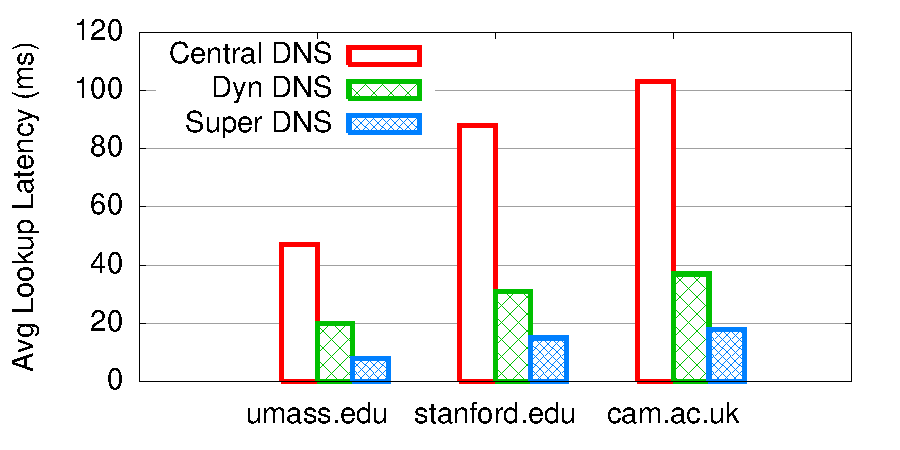
\includegraphics[scale=0.43]{graph/newgraphs/dns.pdf}
%\vspace{-0.15in}
%\caption{Managed DNS provides lower address lookup latencies than centralized authoritative name servers.}
%\label{fig:dnsmanaged}
%\vspace{-0.2in}
%\end{figure}
%
%




















\eat{
\vspace{-0.1in}
\subsection{Why not just adapt DNS?}
{\tiny{
While architectural positions like above are endlessly debatable, a more pressing question is: what if any are the limitations of DNS as a global name resolution service under high mobility and how can it be retrofitted to address those limitations?

The scalability challenge of high mobility would be felt most strongly at the authoritative name servers for two reasons. First, they would need orders of magnitude higher updates rates from mobile device names a couple orders of magnitude more in number compared to domain names today ($\approx$10B vs 146M \cite{gartner}).  Second, authoritative name servers would be unable to take advantage of TTL-based caching for  mobile device names  as much as for today's domain names.  TTLs of A-type records in DNS are more than 5 minutes for more for 40\% of records and more than 1 hour for 10\% of records\cite{Gao2013}, which implies a commensurate service outage time as updates take that much time to fully propagate. In practice, actual update rates to DNS records are orders of magnitude lower than that indicated by TTLs that are set conservatively so as to reduce outage times due to unanticipated updates; yet, ironically, outage times can often last a day or more either because of poorly planned updates or because some resolvers do not respect the TTL limits much to the woe of server administrators \cite{serverfault}. In contrast, mobile devices would require smaller TTLs to ensure reachability and can be expected to make tens of updates per day or more on average (and more frequently in short bursts such as in vehicular WiFi environments \cite{Wiffler}). Smaller TTLs imply higher load. %Due to short TTLs of mobile device names, a high fraction of lookups would reach authoritative name servers and increase their load. 

%Current DNS relies heavily on TTL-based caching to reduce address lookups to authoritative name servers. 



%Is it possible to retrofit current DNS design to provide name resolution for mobile hosts? What, if any, are the performance or scalability constraints that DNS would encounter?
\eat{
The first challenge is scalability. DNS currently manages name records for 146 million domain names \cite{whois}. To support all cell phones and tablets in the world today \cite{gartner}, DNS would have to maintain about two orders of magnitude more name records. Given the effectiveness of DNS's hierarchical and federated design in scaling by several orders of magnitude in the last three decades, one might reasonably assume that supporting more names is simply a matter of provisioning commensurately more resources at different levels of the hierarchy.

However, high mobility really throws a spanner in the works as the key to DNS scalability is its heavy reliance on TTL-based caching throughout the hierarchy. Our measurements as well as those by others suggest that DNS TTLs are more than 5 minutes or more for 40\% of records and more than 1 hour for 10\%  of records \cite{Gao2013}, which implies a commensurate service outage time as updates to resource records take that much time to fully propagate. In practice, actual update rates to DNS records are an order of magnitude lower than that indicated by TTLs that are set conservatively so as to reduce outage times due to unanticipated updates; yet, ironically, outage times can often last a day or more either because of poorly planned updates or because some resolvers do not respect the TTL limits much to the woe of server administrators \cite{serverfault}. In contrast, mobile devices would require small TTLs to ensure reachability and can be expected to make tens of updates per day or more on average, and more frequently in short bursts such as in vehicular WiFi environments \cite{Wiffler}. 

The second challenge is balancing performance and cost at authoritative name servers, the DNS tier that must bear the brunt of significantly higher update rates. 
}
%The effect of short TTLs would be felt most at the authoritative name servers, who would be frequently contacted to get the latest addresses of the mobile device.

%making DNS poorly suited for high mobility.

%To provide name resolution for mobile hosts, DNS would face two main challenges. First is the scale of the workload. DNS currently manages name records for 146 million domain names \cite{whois}. As the number of mobile devices already exceeds 1 billion \cite{gartner}, DNS would be expected to support name resolution for at least an order of magnitude more names that it does today. Given the success of DNS in scaling to a workload of size $10^8$, we expect that another  order of magnitude increase in workload could possibly be handled by provisioning more resources at every level of its hierarchy. 

To handle high mobility, we expect most end-users to outsource their authoritative name service to managed DNS providers. Managed DNS providers today are commonly geo-replicated and allow their customers to leverage better performance, availability, economies of scale, and ease of management compared to maintaining a centralized authoritative name server by themselves. However, managed DNS providers today use simplistic strategies such as {\em replicate-all} or {\em static-k} that respectively replicate a name record at all available locations or a fixed set of packaged locations (e.g. Dyn DNS offers replicate-at-all package for \$180/yr and replicate-at-4  for \$30/yr). We argue that these simplistic strategies provide poor cost-vs-performance tradeoffs even for today's (mostly) non-mobile names, a problem that will be further exacerbated by high mobility.

%Managed DNS services could offer a way to handle load on authoritative name servers.  A geo-replicated managed DNS service would have much better availability and performance than  a centralized authoritative name server.  Managed DNS providers would be able to leverage economies of scale and ease of management and would provide a more cost effective solution for mobile device names.  Desite these advantages, managed DNS providers must still manage much higher update costs of geo-replicating mobile name records. However, managed DNS providers today use simplistic strategies such as {\em replicate-all} or {\em static-k} that respectively replicate a name record at all available locations or a fixed set of packaged locations. For example, Dyn DNS offers a replicate-at-all-locations package for \$180/yr and a replicate-at-4-locations package for \$30/year. These simplistic replication strategies do not provide the best cost-vs-performance tradeoffs as shown  by the following analysis for today's domain names.

%A key cost concern for these providers in seviing mobile names would be orders of higher updates  of maintaining geo-replicated name records. 



%; these update costs are much smaller for today's domain names.
% we take . 
%The cost-vs-performance tradeoffs for managed DNS providers are apparent even today, but mobile devices names would drive up the costs of updating geo-distributed replicas by orders of magnitude, and would require strategies that provide better cost-vs-performance tradeoffs than those offered by simplistic replication strategies. 

%A centralized authoritative name server would have both poorer availability and performance, thereby necessitating a geo-replicated deployment. There would be increasing pressure on mobile device names and even small businesses and organizations to move to managed DNS providers in order to leverage economies of scale and ease of management. Managed DNS providers today employ geo-replicated authoritative name servers in order to reduce lookup latencies for their clients, e.g., twitter.com uses DynDNS \cite{dyndns}.

%could achieve better cost-vs-performance tradeoffs to handle high updates rates of  mobile device names

%To appreciate the benefit of migrating to a managed DNS provider from a centralized authoritative name server and  the limitations of managed DNS providers simplistic strategies, we take examples from today's domain names.  

To exemplify our argument for non-mobile names, consider Figure \ref{fig:dnsmanaged} that shows lookup latencies to centralized authoritative name servers of three domain names (CentralDNS), and their projected lookup latencies for two managed DNS services: (1) Dyn DNS, a leading provider with 17 known locations \cite{dnscompare}  and (2)  SuperDNS, a hypothetical managed DNS with 200 (PlanetLab) locations but replicates a name at only 17 out of the 200 locations where the domain name is highly popular. We calculate latencies based on measurements from 100 other PlanetLab locations. We measure lookup latency for Dyn at a location by querying Dyn servers for the address of twitter.com, one of its customers. The latency of SuperDNS at a location is the measured round-trip delay to the nearest replica of the name record.   We take the weighted average of lookup latencies across all locations weighted by the popularity of a domain in the geographic area (calculated using the Alexa dataset  \cite{alexa}) for which that location is geographically closest.

Unsurprisingly, managed DNS services do improve performance over a centralized service, e.g., Dyn reduces lookup latency for cam.ac.uk by 2.7$\times$. However, its simplistic replication policy leaves significant room for improvement compared to SuperDNS that leverages its massively geo-distributed deployment and intelligent replica placement, to give up to 2.5 $\times$ better performance than Dyn for the same number of replicas.
If SuperDNS were to replicate each name at all 200 locations, its update costs would increase by nearly 12$\times$.  To limit update costs, if SuperDNS were to follow a static-k policy and choose 17  locations randomly,  it would be unable to effectively use its massively geo-distributed deployment to minimize latencies.  Highly mobile device names would further exacerbate the cost-benefit tradeoffs of such simplistic replicated strategies as they would not account for the orders of magnitude higher update costs.
}}

}
%high demand for the  to be in regions of high demand for the domain name.
% that are selected in regions  selected  as per the geo-distribution of demand of the name.

%To appreciate both the benefit of migrating to a geo-replicated managed DNS provider from a centralized authoritative name server as well as the limitations of commercial managed DNS providers today, consider Figure \ref{fig:dnsmanaged}. The figure shows lookup latencies to authoritative name servers of three domain names that use a centralized server (Central DNS), and their projected lookup latencies for two managed DNS services: (1) Dyn DNS, a leading provider with 17 known locations \cite{dnscompare}  and (2)  Super DNS, a hypothetical managed DNS with 200 locations (selected from PlanetLab nodes); Super DNS replicates a name at only 17  locations that are the closest name servers selected  as per the geo-distribution of demand of the name.

%the current single location authoritative name server maintained for that name  and two alternative services: 
% assuming that its other customers would see similar performance.  

%The actual and projected lookup latencies 

% The lookup latency for a service  is the weighted average of  its lookup latencies across all locations; the weight of a location is proportional to the popularity of a domain in the geographic area for which that location is geographically closest.  

%We measure the performance of Dyn DNS at a location based on 

%The  projected performance of the managed DNS services is measured as follows: (a) Dyn DNS:  We measure lookup latency by querying Dyn servers for a domain name of one of its customers  (twitter.com) assuming that its other customers would see similar performance. (b) Super DNS:  We measure round trip latency to the nearest server at which the name record is replicated. 


%service at a location is measured as follows: (a) Central DNS: We measure lookup latencies to the authoritative name servers for the domain name. (b) Dyn DNS:  We measure lookup latency by querying Dyn servers for a domain name of one of its customers  (twitter.com) assuming that its other customers would see similar performance. (c) Super DNS:  We measure round trip latency to the nearest server at which the name record is replicated. The lookup latency for a service  is the weighted average of  its lookup latencies across all locations, where the weight of a location is proportional to the aggregate demand in the region for which that location is the geographically closest.  The geo-distribution of the demand for domain names is obtained from the  Alexa dataset  \cite{alexa}.


%To illustrate another hand-picked example, a small business in Amherst, MA \verb+www.loosegoosecafe.com+ has all four authoritative name servers in Atlanta TBD about 80ms away


%These results exemplify that it is possible to achieve better cost-performance tradeoffs than currently used simplistic replication strategies.
%Although these results are for todays domain names, they exemplify that it is possible to achieve better cost-performance tradeoffs than those offered by simplistic replication policies of today's managed DNS providers. 

%follows a replicate-all policy, it would use all 200 locations for every domain name, which would increase its update costs for keeping consistent replicas by nearly $12\times$. Alternatively, it could follow a static-k policy and choose 17  locations randomly to limit the update cost but in that case, would be unable to take advantage of its massively geo-distributed deployment to minimize latencies. 

 %DNS could be equipped to handle high mobility workloads by migrating to managed DNS services for authoritative name resolution. However, the simplistic replication strategies of today's managed DNS services leave much room for both improving performance and reducing update costs associated with  highly mobile names. 



%A managed DNS service can significantly reduce lookup latency for these domain names compared to their current single-location authoritative name servers, e.g., Dyn DNS reduces lookup latency for cam.ac.uk by 2.5$\times$.  




%
%%Performance that a domain name would see from 100 Planetlab locations if it were to use that service. 
%
%
%The geo-distribution of the demand for that domain name from Alexa dataset \cite{alexa}. For all three services, the latency shown is the weighted average of  lookup latency across all locations, where the weight of a location is proportional to the aggregate demand in the region for which that location is the geographically closest. 
%
%
%\emph{Single-location:} We calculate this latency by measuring DNS lookup latencies to the authoritative name server from 100 PlanetLab locations.  
%
%%To ensure that the average lookup latency reflects the actual geo-distribution of the DNS lookups for that domain name, we obtain city-level demand for that domain name from Alexa dataset \cite{alexa}. 
%
%
%\emph{DynDNS:} We measure the performance of Dyn from the same locations by querying Dyn servers for a domain name (twitter.com) serviced by Dyn. The performance that this domain would see for if it were to use Dyn servers is obtained by taking the weighted average of lookup latency 
%
%\emph{Managed DNS Super:} We select 17 locations that are close to the locations selected by Dyn DNS and are also close to 
%
%
%
%We measure the lookup latencies for twiiter.com domain name serviced by Dyn from PlanetLab location 
%We calculate this latency by measuring DNS lookup latencies to the authoritative name server for that domain from 100 PlanetLab locations. and by taking a weighted average of these lookup latencies based on the geo-distribution of the demand for the 
%
%
%Dyn-DNS






%The second challenge is that authoritative name servers would see many orders of magnitude larger update rates of records for mobile hosts than those seen for current domain names.  This challenge too is addressable if a small number (2-3) of replicas of authoritative name servers are maintained.  The additional update load could be supported by  provisioning more resources at authoritative name servers if necessary. To keep a small number of consistent replicas of an authoritative name server would further inflate the cost by a small factor, and hence could be supported.
%2-3, which is a manageable factor of increase in cost. Thus, for a small number of authoritative name servers, DNS appears to handle this challenge as well. 

% The  key problem with maintaining authoritative name servers at a small number of locations is that address lookups to authoritative name servers take as long as global propagation delays, i.e., hundreds of milliseconds, and result in increased connection setup times. The state-of-the-art solutions for authoritative name servers, managed DNS providers \cite{ultradns, dyndns, dnsmadeeasy}, address this problem by deploying servers at a few tens of locations globally and replicating name records from their customers at all locations.  These providers provide authoritative DNS service for  many of the top enterprises today.
 
% If these providers were to provide authoritative name service for mobile hosts, their current design makes it extremely hard for them to provide  a cost-effective, and high performance  service due to following reasons:
 
%The current design of managed DNS providers makes it extremely hard for them to provide  a cost-effective, and high performance  service for all mobile hosts in the Internet. These providers would incur excessively high update cost at each location due to their policy of replicating name records at all locations. For example, processing 100M updates/sec from 10 billion mobile devices alone would require thousands of machines to be deployed at every location. This "replicate-everywhere" policy entails that the deployment consists of a small number of locations each of the size of a large data center. Thus, due to high update costs associated with adding new locations, it would be much more costly to maintain even their current deployment of tens of locations across the globe;   and  infeasible to have a massively geo-distributed deployment at hundreds or thousands of locations, e.g. Akamai's servers are deployed at more than 10000 locations, that provides small lookup latencies (few ms) to users across the globe. 

%While high mobility of end-hosts makes it costlier to have more deployments, managed DNS providers do have considerable room for reducing lookup latencies with a more geo-distributed deployment of servers. We measured the address lookup latency to authoritative name servers for 318 domain names that are serviced by a leading managed DNS provider. These measurements were done from 100 PlanetLab locations by sending a total of 1000 lookups for each domain name across all locations. Figure \ref{fig:lookuplocation} shows the distribution of median lookup latencies at all locations. Lookup latency is more than 100 ms from  30\% percent of the locations. This finding suggests that the current deployment of managed DNS providers, due to a limited geo-distribution of their servers, does not fully address the problem of high lookup latencies to the authoritative name servers.



%\begin{figure}
%\centering
%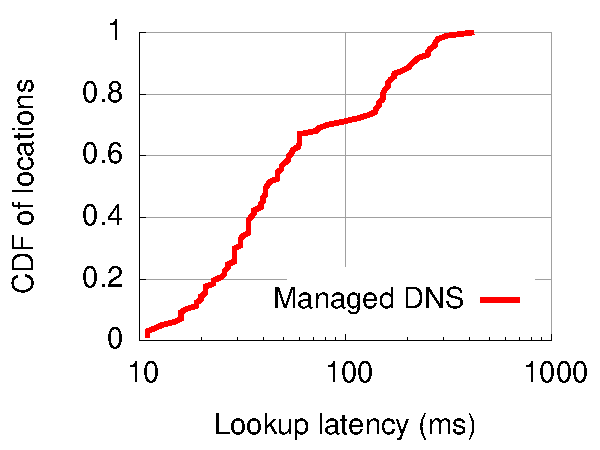
\includegraphics[scale=0.5]{graph/newgraphs/lookup-location.pdf}
%\vspace{-0.1in}
%\caption{Distribution of latency of lookups to authoritative name servers of a managed DNS provider from 100 Planetlab locations.}
%\label{fig:lookuplocation}
%\vspace{-0.1in}
%\end{figure}


% from 100 PlanetLab locations to authoritative name servers  for 318 domain names that are serviced by a leading managed DNS provider (refer to Section \ref{sec:managed}). 
%This finding suggests that managed DNS providers have considerable room for reducing lookup latencies with a more geo-distributed deployment of servers.

%In summary, the current DNS design could be used to provide name resolution for mobile hosts but would continue to face the problem of high lookup latency to the authoritative name servers. Having a massively geo-distributed deployment of authoritative name servers could provide low lookup latencies across the globe, but prohibitively high update costs associated with mobility makes it infeasible for managed DNS providers to support such a deployment in a cost-effective manner.


%
%
%
%For the name records of mobile hosts, authoritative name servers would see an update rate that is orders of magnitude higher than those of currently existing records in DNS.  over-provision authoritative name servers to solve the problem. 
%Second problem, which plagues name DNS even today is that lookups to authoritative name servers results in high latencies. 
%
%



%%%%%%%%%%%%%previous version of this section%%%%%%%%%%%%%

\eat{
Providing name resolution for mobile hosts would present DNS with a workload with very different characteristics than that of today's DNS.
For the name records of mobile hosts, authoritative name servers would see an update rate that is orders of magnitude higher than those of currently existing records in DNS. 
Frequent address updates by mobile hosts imply that cached addresses could be reused for much shorter durations. A record for a user that changes networks 100 times a day could be reused only for 15 minutes on average, after which a fresh name record must be fetched from the authoritative name servers. Frequent lookups to authoritative name servers, besides increasing the load on authoritative name servers, would increase connection setup time to mobile hosts. For example, if the authoritative name server is maintained at a single location, address lookups may take of the order of global propagation delays, e.g., 100s of milliseconds. Increased load of lookups and updates on authoritative name servers could be managed by provisioning more resources at authoritative name servers, but high lookup latency to authoritative name servers remains the primary problem for current DNS.
%Therefore,  is a challenge, even though provisioning  more resources at authoritative name servers could help cater to an increased load.


The state-of-the-art solutions for authoritative name servers are provided by managed DNS providers. These providers maintain servers at a few tens of locations globally and replicate name records from their customers at all locations.  These providers handle the DNS service on behalf of many of the top enterprises today. 
However, the currently available the managed DNS provider solutions have two main shortcomings: 

(1) Due to a limited geo-distribution of their servers, managed DNS providers do not fully address the problem of high lookup latencies to the authoritative name servers. We measured lookup latency to authoritative name servers for 318 domain names that are serviced by a leading managed DNS provider from 150 PlanetLab locations. Figure 1 shows the distribution of lookup latencies in our measurements. 30\% percent of lookups take more than 100 ms. 
%authoritative name servers managed DNS providers from 150 PlanetLab locations to 318 domain names in the top 10K websites as per Alexa ranking; these names are served by a leading managed DNS provider.

%For instance, to connected to a mobile host who is 10 ms away, may need a lookup that is 150 ms or even more.


(2) These providers would incur excessively high update cost at each location due to their policy of replicating name records at all locations. For example, processing 100M updates/sec from 10 billion mobile devices alone would require thousands of machines to be deployed at every location. This "replicate-everywhere" policy entails that the deployment consists of a small number of locations each of the size of a large data center. Thus, due to high update costs associated with adding new locations, it is infeasible to have a massively geo-distributed deployment at thousands of locations, e.g. Akamai has 10000 locations, that provides small lookup latencies to users across the globe. 

In summary, the current DNS design is ill-suited to provide name resolution for mobile hosts due to high lookup latencies to authoritative name servers. Having a massively geo-distributed deployment of authoritative name servers could provide low lookup latencies across the globe, but prohibitively high update costs preclude such a deployment. 
}
